%Empieza configuracion de capitulo

\setstretch{1.0} \titleformat{\chapter}[block]{\Large\bfseries}{CHAPTER
\Huge\thechapter\vspace{25 pt}}{0 pt}{\\\fontsize{26}{36}\selectfont}
\titlespacing{\chapter}{0 pt}{30 pt}{50 pt}[0 pt]
\titleformat{\section}{\Large\bfseries}{\thesection}{0 pt}{\hspace{30 pt}}
\titleformat{\subsection}{\large\bfseries}{\thesubsection}{0 pt}{\hspace{30
pt}} \pagestyle{fancy} \fancyhead[LO,LE]{\footnotesize\textit{\leftmark}}
\fancyhead[RO,RE]{\thepage} \fancyfoot[CO,CE]{}
%Termina configuracion de capitulo

\chapter{Introduction} %Cambia Introducci'on al nombre de tu capitulo
\setstretch{1.5} %Regresa el interlineado a 1.5

\normalsize This work presents a detailed study of how within a network of
embedded systems, computing devices collaborate within each other to solve
parallel problems. At the end a detailed case of study based on industrial
benchmarks for distributed systems, power consumption analysis and optimal
operating system selection, describes a methodology to maximize power
efficiency.

\section{Background} \vspace{30 pt} \noindent

The evolution of computing technology has made an incredible progress since the
first general-purpose electronic computer was created. Today, less than 300
dollars will purchase a personal computer that has more performance, more
memory, and more disk storage than a computer bought in 1985 for 1 million
dollars\cite{Hennessy}. Incredible advances have been possible thanks to
innovations in computer and software design. 


%Computter architecture
Since the commercial use of computers (started in 1951 with the introduction of
UNIVAC \cite{Nur}) the development of computers has had multiple changes, not
only from the architectural point of view but also from the application point
of view. In \cite{Hennessy} the authors present the evolution of the computers
in term of performance over the years since 1980. The first important
breakpoint in the history of computers came in the beginning 1970s whit the
emergence of the microprocessor. 

The 1980s saw the rise of the desktop computer based on microprocessors, in the
form of both personal computers and workstations. The 1990s saw the emergence
of the Internet and the World Wide Web, the first successful laptop computing
devices, and the emergence of high performance computing systems for business
purposes (servers). During these years the performance of the microprocessors
increase around 27\% each year \cite{Hennessy}.

However, in the first years of the 2000 decade a dramatic change in the
computer architecture happened. The idea of increasing computing performance in
processors, based mainly on increasing the clock frequency, could not longer be
held. This is due to the fact that the power density (amount of power per
volume unit) is multiplied with increases in frequency. 

The solution, to keep meet Moore's \cite{Mack} law, was shifting to real parallelism by
doubling the number of processors on the die. This was the birth of multi-core
microprocessors area. The idea consider increasing the computing performance
by limiting the power density at the same time. This new computer architecture
broke the paradigm of using small microprocessors for embedded platforms.
Instead of this it was possible to have more computing power with less
frequency. Thanks to this radical change there has been a rapid evolution of
the computing and multimedia capabilities on embedded systems. 


%Embedded architecture
According to \cite{Hallinan}  \textit{"An embedded system is a special-purpose
system in which the computer is completely encapsulated by the device it
controls"} Unlike a general-purpose computer, an embedded system performs
pre-defined tasks, usually with very specific requirements. Examples of these
are: microwave ovens, washing machines, printers, and GPS (Global Positioning
System) systems. All those electronic based appliances that started to emerge
around 35 years ago \cite{Nur}. 

The variety of embedded applications requires a wide spread of processing power
and cost. They include 8-bit and 16-bit processors that may cost few cents,
32-bit microprocessors that execute 100 million instructions per second and
cost few dollars, and high-end processors for the newest video games
or network switches that cost at least 100 dollars and can execute one billion
of instructions per second \cite{Hennessy}.

%Ubicuos systems
Continuous design tradeoffs of factors like: cost, size, power density,
performance and connectivity has caused the computing technology to evolve
rapidly, today ubiquitous computing is a reality. According to Mark
\cite{Mark}, ubiquitous computing is \textit{"the method of enhancing computer
use by making many computers available throughout the physical environment, but
making them effectively invisible to the user"}. This means that computing
power could be made available anywhere and at any time. 


%IoT
According to \cite{Nur}, there is a transformation from ubiquitous computing to
advanced ubiquitous computing. Advanced ubiquitous computing is an extension of
ubiquitous environment that improves connectivity between devices. The main
characteristics of such environment can be listed as follows: a large number of
heterogeneous devices, new communication technology, and Internet of Things
(IoT) among others.

One of the most accurate definitions of IoT given by \cite{Bahga} where it
mentions that \textit{"Internet of Things refers to physical and virtual
objects that have unique identities and are connected to the Internet to
facilitate intelligent applications"}. IoT enables interconnection, via the
Internet, of computing devices embedded in everyday usage objects, enabling
them to send and receive data. Differences respect to traditional embedded
systems include Internet connectivity and smaller power consumption. IoT
systems must always be connected to the Internet and require lower power
consumption. An IoT solution has the following parts (figure~\ref{fig:1.1}).


\begin{itemize} 

\item The Thing (computing devices): In the Internet of Things, a thing can be
any natural or man-made object that can be assigned a unique identifier and
provided with the ability to transfer data over a network. 

\item Network Connection: Network Connections provide connectivity between
computing devices and the Internet, a network, or another computing device. 

\item Cloud Computing data centers for storage and big data analysis: The data
by itself is not useful to the end user. After data is sent and stored into the
cloud computing data centers is necessary to run big data solutions that
present meaningful information to users. 

\item Presentation Devices: Dashboards have to be hosted on some kind of
display, it could be a desktop computer running an application, a tablet, or a
smart phone accessing to a web page. It could even be a purpose-built device
like a retail kiosk, an intelligent vending machine or a control panel. The
goal is to present information coming from the big data analysis. 

\end{itemize}

\begin{figure}[H] \centering
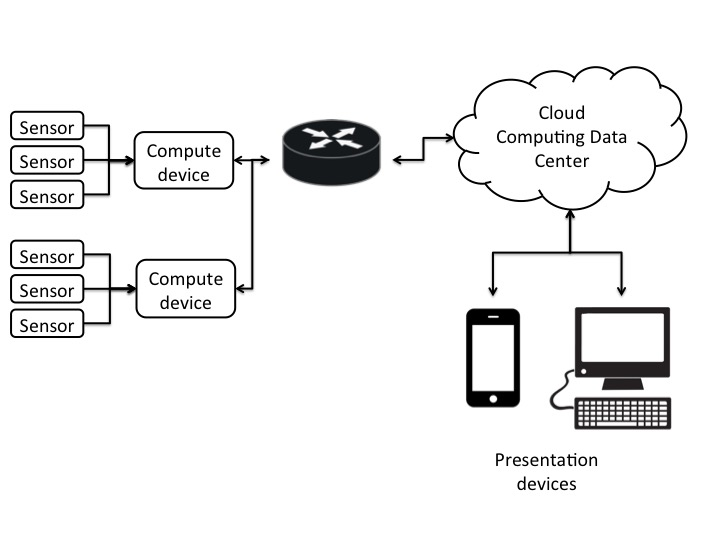
\includegraphics[width=1\textwidth]{images/IoT_diagram.jpg} \caption{An IoT
system diagram } \label{fig:1.1} \end{figure}

The IoT revolution lacks of industry standards. There are thousands of
computing devices and sensors from different vendors that appear on the market
every day, each one with its unique way to send or store data in centralized
cloud computing centers. 

There are two main projects that are organizing information to establish
standards for IoT communications: 

\begin{itemize}

\item Open Connectivity Foundation (OCF)\cite{Terry}: The OCF tries to create a
set of open specifications and protocols to enable devices from a variety of
manufacturers to securely and seamlessly interact with one another. Regardless
of the manufacturer, operating system or chipset the devices that adhere to the
OCF specifications should communicate together. 

\item AllSeen Alliance (before known as AllJoyn) \cite{Massimo}: Is an open
source project for the development of a universal software framework aimed at
the interoperability among heterogeneous devices, dynamic creation of proximal
networks and execution of distributed applications. The framework provides a
common interface towards smart devices.

\end{itemize}

Both standards try to solve a simple problem: To establish communications
standards among the industry. This means that all IoT devices could communicate
with each other in spite of the vendor type. Regardless of these, none has
defined a common standard in terms of IoT technology. 

On the other side we daily use computerized technology like: air conditioners,
televisions and cars; many of them connected to the Internet, In spite of the
existing efforts to develop standard network protocols for IoT systems there is
no one to make the IoT systems analyze their data on their own , instead of
sending all data to cloud data centers for analysis. This is a problem in the
short term because the solution might require to add another server (which may
have space and economic constrains).



\section{Problem Definition} \noindent

The use of IoT devices is rising quickly, according to \cite{Benkhelifa}, by
2022 is it expected to have 14 billions of IoT devices creating a rise of
data processed, transmitted and stored. Considering a scenario where all those IoT
devices would try to send 1 kilobyte of data to centralized servers at the same
time; it would create so much traffic that would be similar to a security
attack \footnote{ In the DDoS attack, high amount of network traffic with
maximum performance are generated and transmitted  to the target
systems\cite{Yang})}, that would collapse centralized data centers.

Apart from the problems of transmitted data, power consumption of
computing systems that store and process data generated by IoT devices
is important to be studied. If current trends continue, a system to handle
IoT data would require 100 megawatts. \cite{Xizhou} \footnote{Millions of
watts, which translates into power for hundreds, and even thousands, of
homes.\cite{Kenward}}. 

Despite of the variety of IoT applications, like those mentioned in
\cite{Liu-Dan} \cite{Du}, all of them are based on the same IoT principle of
sending data over the Internet to a centralized processing system without using
the processing capabilities of the IoT device.  In many IoT designs \cite{Du}
a dedicated microprocessor is used to transmit data to the centralized
control system; regardless that the logic of the centralized control system is
just a simple conditional rule. On the other hand, there are very few examples,
like those listed in \cite{Wun}, where the computing power of the embedded
platforms is exploited. If the IoT industry continues creating solutions
without optimizing the use of the computing power of the embedded platform
sending data over the Internet; then more critical examples as that of Boeing
787\textregistered\  \footnote{ The Boeing 787\textregistered\ aircraft ordered
by Virgin Atlantic\textregistered\  for delivery dramatically increases the
volume of data the airline will need to deal with (half terabyte in a
transatlantic flight). Because they can't handle that much terabytes of data
everyday coming from various airplanes they are looking for adding servers
inside the airplanes \cite{Virgin}} will be seen.

This research work proposes a method to improve the use of all IoT platforms by
reducing the amount of data transmitted, as well as, the amount of high
performance servers needed for data processing. 


\section{Main Objective} \noindent

The main objective of this work is to show how an IoT network could be self
sustainable. It means to make it solve their own computing problems without the
need to send data to data centers (or to the cloud). The work will study when
is necessary to send data to data centers or the cloud.
It will estimate the maximum number of embedded platforms that provide the
maximum level of performance with the minimal amount of power consumption. At the
same time, a list of applications that are good candidates for that approach is
presented. 

This work intends to provide to the IoT industry a way  to determine whether
applications can take advantage of the communication between  IoT devices
to process their own data instead of sending information to data centers.

\section{Hypothesis} \noindent

On recent years it has been observed that unsustainable power consumption has
driven the microprocessor industry to integrate multiple cores into a single
die, or multicore, as an architectural solution in order to increase
performance and reduce power density. The same approach might be followed for
IoT systems by creating a self sustainable network of IoT systems, where
processing could be solved with parallel computing technology and distributed
clusters).

With the current computing power of ultra-low-voltage microprocessors
platforms (which are core systems of the IoT devices) it is possible to create a cluster
with the optimal number of embedded platforms. All interconnected in a
network that provides maximum performance with small
power consumption. This characteristic is determined by power efficiency of
the network. The power efficiency is quantified by performance per watt
\cite{Jun}.

The key result is to determine at what point it is better to send data to data
centers. This consist on finding what is the maximum number of systems that
this kind of network can handle with optimal energy efficiency.

The development of metrics to evaluate energy efficiency on the basis of
performance and power models is described in \cite{Dong}. According to
\cite{Dong}, the formula for performance per watt (Perf/W), which represents the
performance achievable at the same cooling capacity \footnote{Cooling
Capacity refers to the amount of cooling that system can remove. It is measured as the
number of BTUs per hour of heat that the unit can remove from the air. (A BTU
or British Thermal Unit). It can also be measured as Watts per hour or tons (
the amount of water at a given temperature that can be frozen in a given amount
of time) \cite{Siegenthaler} } (Watts/h) based on the average power
(\textit{W}) is shown bellow in \ref{eq:1}:

\begin{equation}\label{eq:1} \frac{Perf}{W} = \frac{1}{(1 + (n -1 ) k (1 - f))}
\end{equation}

According to Amdahl's law\cite{Dong}, the formula for computing the theoretical
maximum speedup (or performance) achievable through parallelization is as
follows: 

\begin{equation}\label{eq:2} Perf = \frac{1}{(1 -f) + \frac{f}{n}}
\end{equation}

Where \textit{n} is the number of processors,  \textit{f} is the fraction of
computation that can be parallelized ( a value from 0 to 1 ) and \textit{k}, to
represent the fraction of power the processor consumes in idle state  ( a value
from 0 to 1 ).

In \cite{Dong} it is demonstrated that a symmetric many-core
processor can easily  lose its energy efficiency as the number of cores
increases. To achieve the  best possible energy efficiency, it is 
suggested a many-core alternative, featuring many small, energy-efficient cores
integrated with a full-blown processor. It is shown that having knowledge of
the amount of parallelism available in an application prior to execution, it is
possible to  find the optimal number of active cores to maximize performance
for a certain given cooling capacity and energy in a system.

In this thesis work it is proposed the hypothesis that a cluster of ultra-low
power IoT platforms can be as computing powerful and energy efficient as the
system described in \cite{Dong}, but in this case \textit{n} is the number of
ultra-low power platforms instead of processor cores.

Results of a simulation to illustrate such hypothesis is described in
Figure~\ref{fig:1.2}.  At the beginning, the increment in the number of nodes
in the studied network produces an increment on performance; however, it is
expected to reach a maximum point at which power efficiency becomes stable and
it will remain in such state up to a certain point at which it will start to
decrease. Such behavior is expected, as the number of platforms increases it is
expected to get some performance benefit, because the amount of work to be done
is distributed among different platforms, but as more are added due to the
power they consume the performance gain starts to minimize. When the ideal
number of platforms is exceeded, the power efficiency decrease rapidly.

\begin{figure}[H] \centering
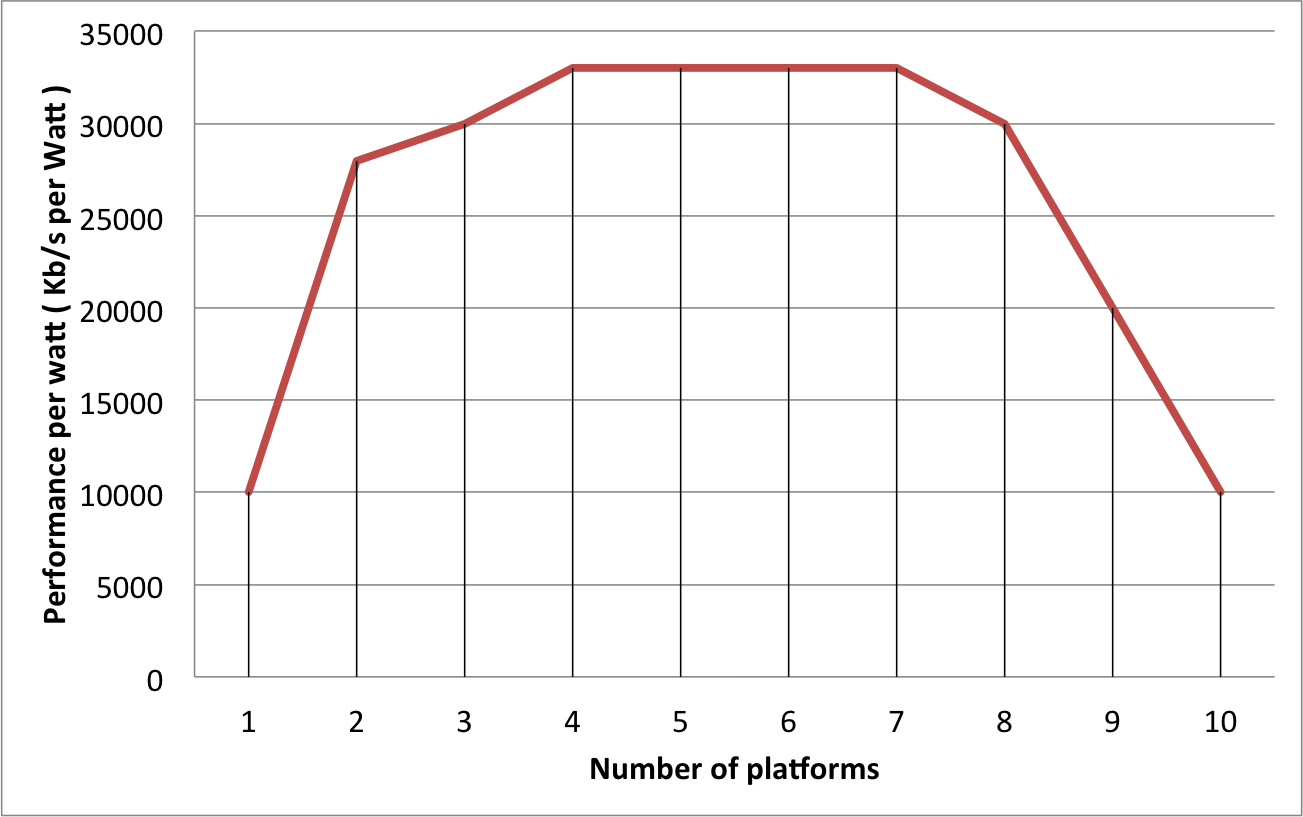
\includegraphics[width=1\textwidth]{images/hypothesys.png}
\caption{Hypothesis of energy efficiency behavior in embedded cluster}
\label{fig:1.2} \end{figure}

After finding these curves for command benchmarks it will be easy for the
industry of IoT systems to determine if their applications can take advantage
of communicate their IoT devices among each others instead of sending the
information to their data centers.

\section{Methodology} \noindent

In this work it is investigated the number the number of platforms to obtain
the best power efficiency for a given set of benchmarks. Recent research work 
\cite{Saldana} \cite{Abgaria} \cite{McMahon} \cite{Liu} demonstrate an
increasing interest in the topic. Such work focuses on three main fields:

\begin{itemize} 
    \item Study of low-voltage platforms with large computing power.
    \item Study of Operating Systems for IoT platforms
    \item Workload balancing schemes for embedded platforms
\end{itemize}

The methodology proposed in this work includes the following steps:

\begin{itemize}

\item To select the correct embedded platform: There are dozens of embedded and
IoT platforms, this is required  to analyze and select the best platform.

\item To select a set of benchmarks. Is important to identify a set of
benchmarks that covers a variety of IoT applications.

\item To select an Operating System for the system 

\item To create embedded clusters for energy efficiency measurements. This
consist of the integration of selected hardware, operating system and computing
paradigm.

\item To find the optimal number of embedded systems in the cluster that
provides the highest power efficiency. 

\item To release improvements and disagreements as open source. 

\end{itemize}

\clearpage
